\mysection{電流帰還バイアス回路の動作点設定}
電流帰還バイアス回路は、エミッタ接地増幅回路の基本形であり、増幅回路の直流電流動作点を決めるための動作原理図である。(実際にこの形のままで使われることはない。)
固定バイアス、自己バイアス等、入力信号(電圧)にバイアスを加える方法はいくつかあるが、一般的に、トランジスタの持つ特性により動作に悪影響を受ける。(直流電流増幅率の温度変化)
この回路は、温度変化による影響を受けにくい設計となっている。

\begin{description}
  \setlength{\parskip}{0cm} % 段落間
  \setlength{\itemsep}{0cm} % 項目間
  \item[ゴール] 前章で決めた動作点と諸条件から直流電流の動作点を決める。(ブリーダ抵抗の値を決定する。)
  \item[キーワード] ブリーダ抵抗、温度補償
  \item[ストーリー] 前章で決めた動作点+諸条件 → 閉路方程式を立てて回路に流れる直流電流を求める。→ 直流電流の動作点を決める。→ LTspice上で設計 → DCスイープにより動作点を確認 → 計算値と比較
\end{description}

\mysubsection{演習手順}
\subsubsection{DC動作点解析}
\begin{description}
  \setlength{\parskip}{0cm} % 段落間
  \setlength{\itemsep}{0cm} % 項目間
  \item [課題7] 図\ref{current_bias_dc}の回路を作成し、.opディレクティブを用いてDC動作点解析をして下さい。(用いた回路図とディレクティブを示すこと。図 6(a)(b))
  DC動作点が正しく設定されているかどうか考えて下さい。
  \begin{figure}[htbp]
    \begin{center}
    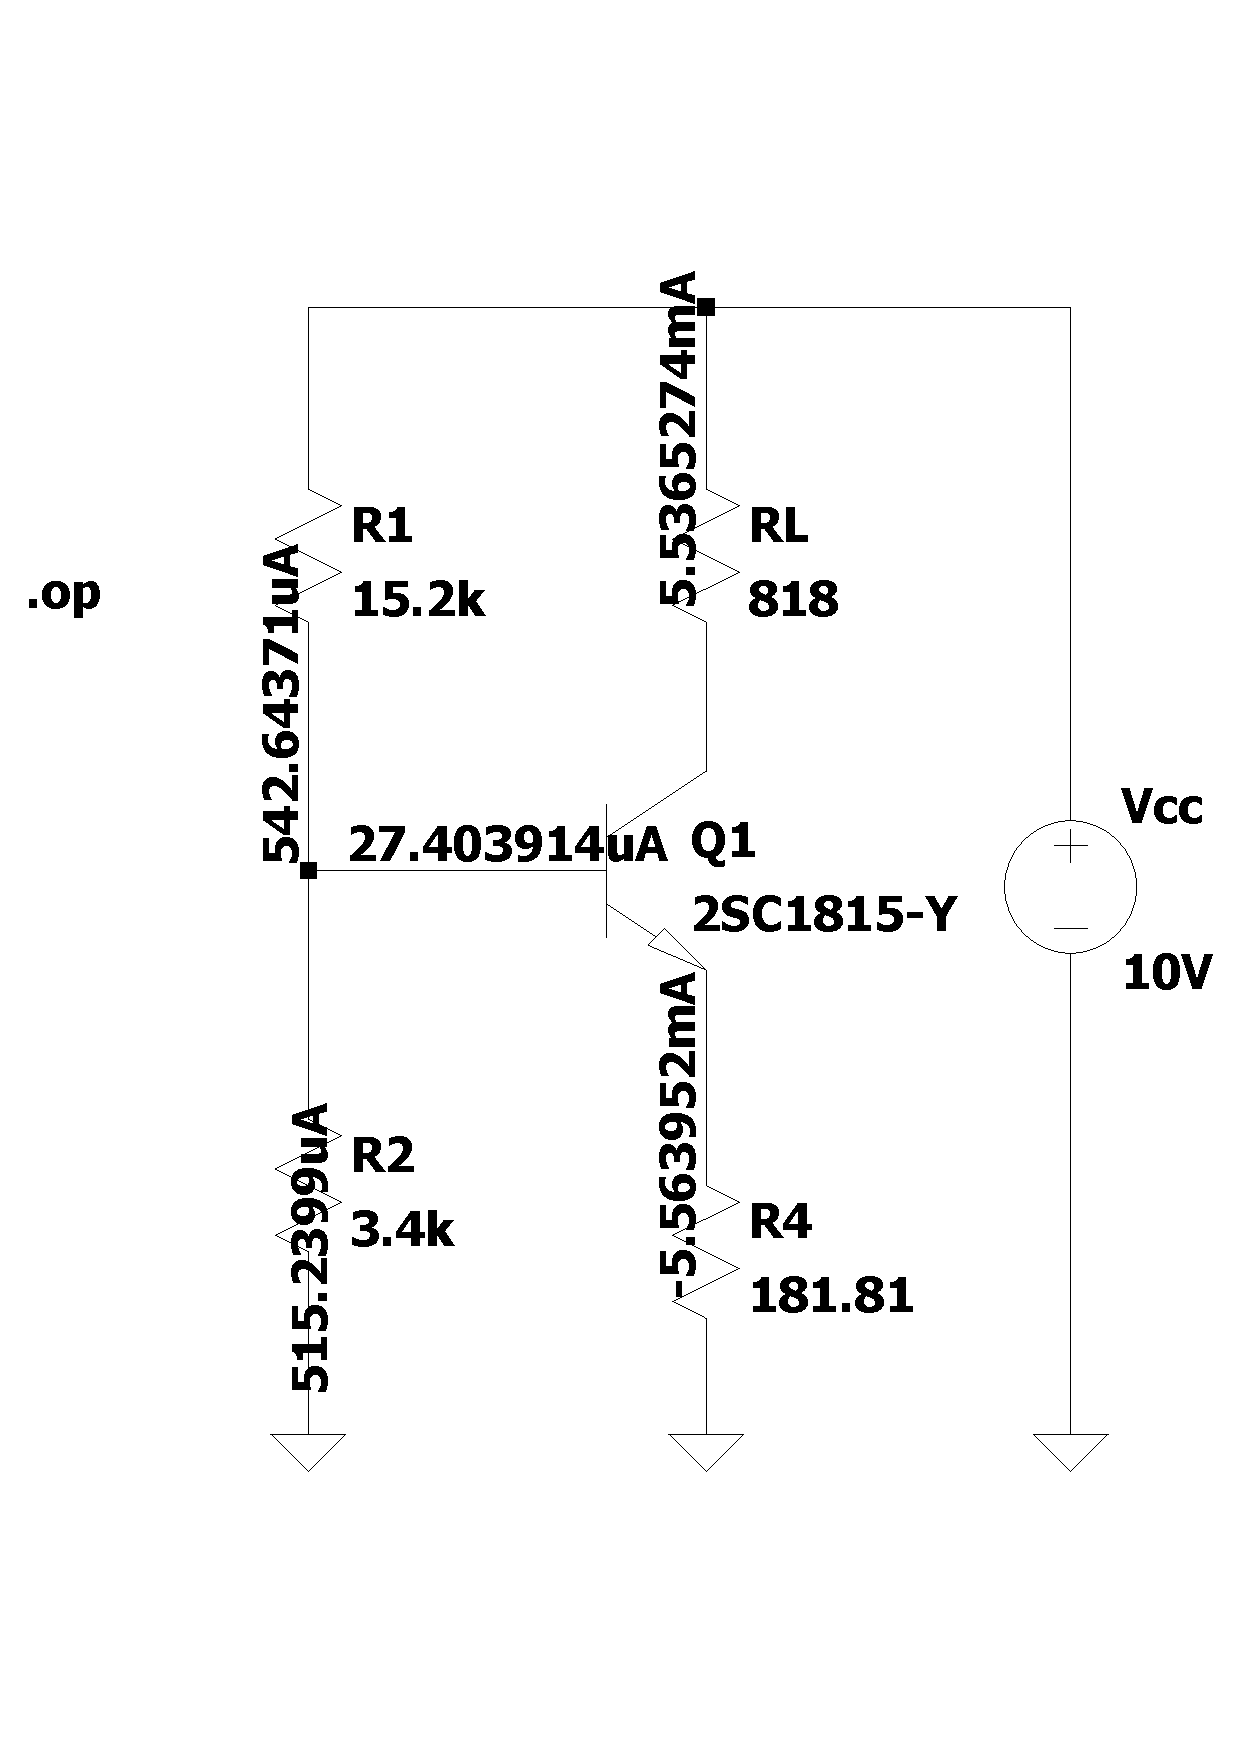
\includegraphics[width=.5\linewidth]{img/44.pdf}
    \caption{電流帰還バイアス回路DC動作点解析}
    \label{current_bias_dc}
    \end{center}
  \end{figure}
\end{description}